\documentclass[10pt,a4paper,titlepage]{article}
\usepackage[utf8]{inputenc}
\usepackage{polski}
\usepackage{amsmath}
\usepackage{amsfonts}
\usepackage{amssymb}
\usepackage{graphicx}
\usepackage{float}
\usepackage{indentfirst}
\author{Adrian Frydmański, Dawid Gracek}
\title{Systemy Inteligentnego Przetwarzania\\--- Projekt ---\\Wahadło odwrócone (sieć neuronowa)}
\begin{document}
	\maketitle
	\clearpage
	\section{Wstęp teoretyczny}
	Odwrócone wahadło niewiele różni się od swojego ,,zwykłego'' odpowiednika. Jest swobodnie wiszącym prętem przymocowanym jednym końcem do wózka. Wózek z kolei ma możliwość poruszania się wzdłuż osi (w jednym wymiarze, acz nic nie stoi na przeszkodzie, żeby rozszerzyć problem wahadła do dwóch wymiarów). Układ ten:
	\begin{itemize}
		\item posiada dwa punkty równowagi: stabilny, kiedy wahadło spoczywa w położeniu dolnym i niestabilny, kiedy wahadło skierowane jest pionowo ku górze,
		\item jest tzw. obiektem niedosterowanym, ponieważ wielkości sterowanych możemy wyróżnić więcej niż jest wejść w układzie.
	\end{itemize}

	\begin{figure}[H]
		\center
		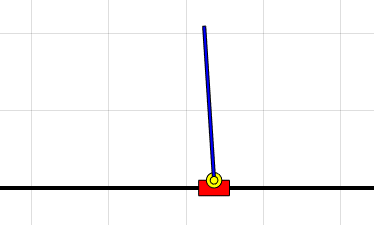
\includegraphics[width=.6\textwidth]{w.png}
		\caption{Model wahadła}
	\end{figure}
	
	Jedyną wielkością, która wpływa na stan układu jest siła przyłożona do wózka, którego przemieszczanie się wprawia w ruch wahadło. Taki układ regulacji może mieć kilka celów:
	\begin{itemize}
		\item stabilizacja wahadła w położeniu górnym,
		\item regulacja położenia wózka w odniesieniu do całego stanowiska,
		\item realizacja algorytmów umożliwiających rozbujanie wahadła z pozycji dolnej i doprowadzenie go to pozycji górnej.
	\end{itemize}
	
	Ów projekt zakłada realizację 2. pierwszych celów poprzez generowanie odpowiednich nastaw regulatora kontrolującego ruch wózka i wprowadzenie go do położenia górnego ze stanu początkowego, gdy wahadło jest nachylone względem ziemi pod kątem mniejszym, niż $90^\circ$. Nastawy mają być generowane przez wyuczoną sieć neuronową.
	
	Matematyczny model wahadła jest opisany na stronie jtjt.pl\footnote{http://jtjt.pl/www/pages/odwrocone-wahadlo/LMIP.pdf} i stamtąd właśnie zaczerpnięte są obliczenia, z których korzysta symulacja.
	
	\section{Implementacja}
	Środowisko, w jakim została przeprowadzona symulacja i tworzenie sieci neuronowej, to Matlab R2017a. Dane testowe do uczenia sieci zostały pozyskane przez funkcję\footnote{Model i funkcja dostępne na https://github.com/Jarczyslaw/Inverted-Pendulum} do strojenia regulatora liniowo kwadratowego w zależności od ,,parametrów środowiska'':
	\begin{itemize}
		\item masa wózka,
		\item masa wahadła,
		\item długość od mocowania do środka ciężkości wahadła,
		\item współczynnik tarcia wózka.
	\end{itemize}
		
	W głównej funkcji, \texttt{lqr\_training}, zostało wygenerowane 100.000 losowych zestawów danych i znaleziono dla każdego z nich odpowiednie nastawy regulatora.\footnote{Cały kod dostępny w repozytorium https://github.com/Adrian94F/SIP} Następnie w narzędziu \texttt{nntraintool} została wygenerowana sieć neuronowa, która na owych zestawach nauczyła się dobierać parametry regulatora. Sprawdzono, że dla 4 neuronów --- tylu, co wyjść --- sieć działa wystarczająco dobrze. Sieć posiada jedną warstwę ukrytą. Przyjęto następujące wielkości podzbiorów zbioru 100.000 zestawów testowych:
	\begin{itemize}
		\item 70\% --- zbiór uczący
		\item 15\% --- zbiór walidacyjny
		\item 15\% --- zbiór testowy
	\end{itemize}
	
	Warto przyjrzeć się dokładniej kilku aspektom, które udało się zauważyć podczas tworzenia niniejszego projektu. 
	
	Mając 4 neurony wejściowe i wyjściowe sieci neuronowej, jej dokładność, czyli wielkość błędu średnio kwadratowego, zależy od przedziału wartości neuronów wejściowych. Zwiększając ten zbiór o jeden rząd dla dwóch neuronów (masy wózka i wahadła), liczbę danych uczących powinno się zwiększyć o 2 rzędy --- jeśli granice badanej przestrzeni zwiększymy w 2 wymiarach 2-krotnie, to by zachować to samo zagęszczenie, należy zwiększyć liczbę elementów w niej 2-krotnie dla każdego wymairu, zatem 4-krotnie. Nie zwiększając go, błąd ulegnie powiększeniu ze względu na zbyt mały rozmiar zbioru danych uczących.
	
	Biorąc po uwagę szybkość generacji danych uczących oraz szybkość uczenia się sieci neuronowej, należy zauważyć, że przedział wartości masy wózka i masy wahadła oraz liczba próbek danych uczących muszą być dostosowane do mocy obliczeniowej i czasu, jaki chcemy przeznaczyć na cały proces.
	
	Dla 100 000 próbek wyznaczono eksperymentalnie, że wartości ograniczające przedział masy wózka i wahadła muszą od siebie odstawać maksymalnie o 3 rzędy. Np. 1 -- 100, 0.1 -- 10 itp. Liczba wartości w przedziale zależy od dokładności funkcji losującej \emph{rand()}, a ta w Matlabie ma dokładność 0,0001.

	\begin{figure}[H]
		\center
		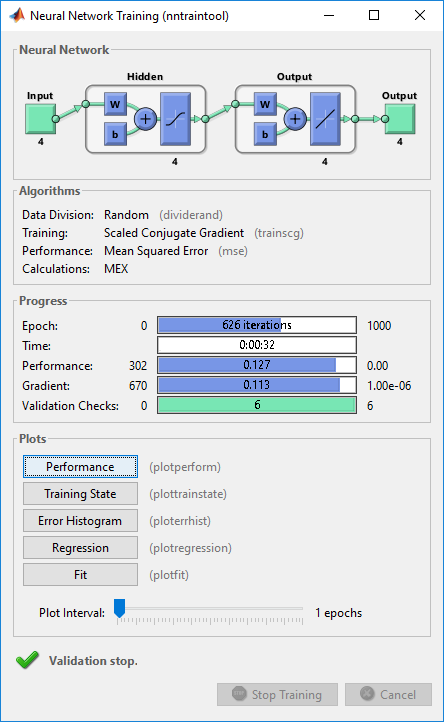
\includegraphics[width=\textwidth]{nn.png}
		\caption{Wygenerowana sieć i proces uczenia}
	\end{figure}

	\begin{figure}[H]
		\center
		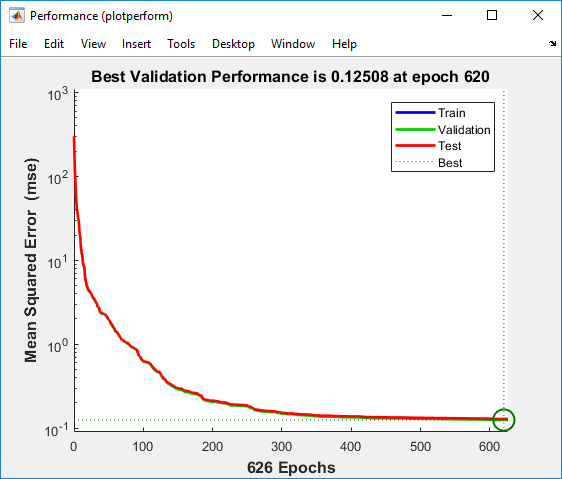
\includegraphics[width=.88\textwidth]{perf.png}
		\caption{Wykres błędów od epok treningowych}
	\end{figure}

	\begin{figure}[H]
		\center
		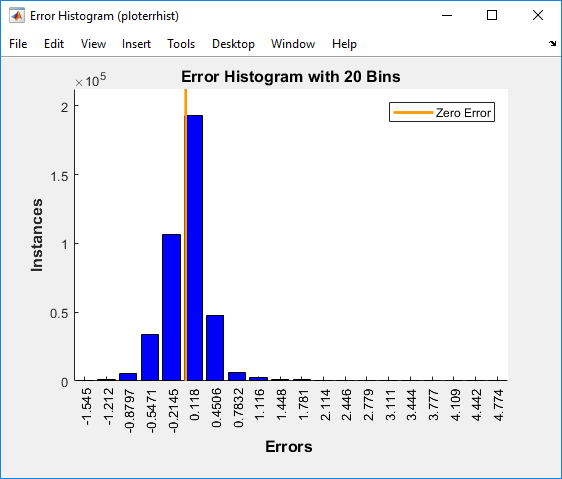
\includegraphics[width=.88\textwidth]{errhist.png}
		\caption{Histogram błędów}
	\end{figure}
	
	Po wygenerowaniu sieci został ponownie wylosowany zbiór zmiennych środowiska, na podstawie których sieć znalazła odpowiednie nastawy regulatorów. Została uruchomiona symulacja i przebiegła ona pomyślnie.
	
	\begin{figure}[H]
		\center
		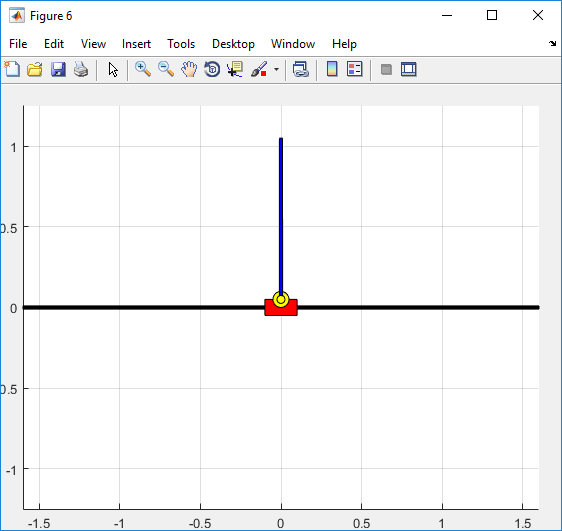
\includegraphics[width=\textwidth]{wyniksymulacji1.png}
		\caption{Osiągnięty stan równowagi podczas symulacji}
	\end{figure}

	\begin{figure}[H]
		\center
		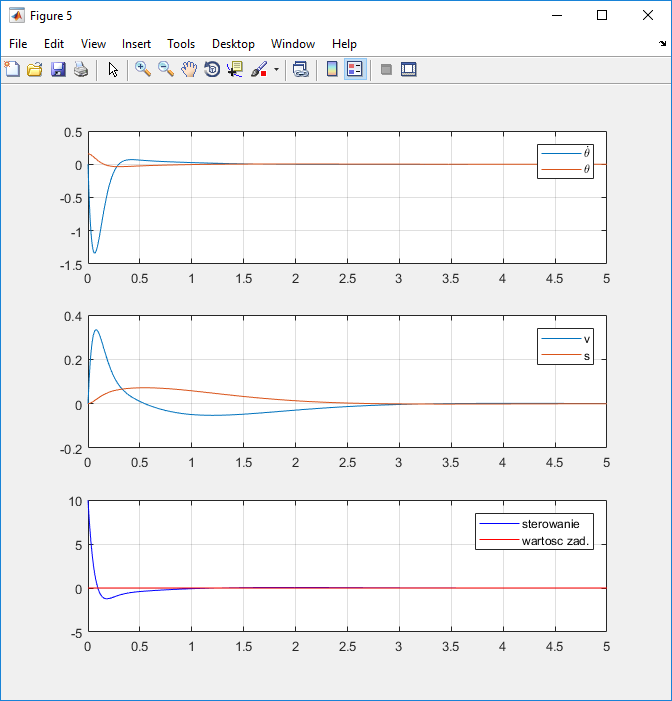
\includegraphics[width=\textwidth]{wyniksymulacji2.png}
		\caption{Wyniki symulacji (od góry): kąt i pochodna kąta pomiędzy wahadłem, a pionem, prędkość i pozycja wózka, przyłożona siła do wózka i zadana wartość zadana}
	\end{figure}
	
	\section{Podsumowanie}
	Projekt pokazał, że sieć neuronową można zaprząc do przeróżnych zadań, nawet do dostosowywania nastaw regulatora w wahadle odwróconym. Jest to możliwe do zrobienia i proste w implementacji w takim środowisku, jak Matlab, aczkolwiek zdaniem autorów projektu zbędne, gdyż funkcja strojąca regulator, dzięki której uzyskano dane do nauki sieci, istnieje i działa wystarczająco szybko. Nie widać więc potrzeby wymiany jej na sieć neuronową, której wynik zawsze będzie obarczony pewnym błędem w stosunku do wyniku działania owej funkcji.
	
\end{document}